\chapter{Development of a Simple Compiler}

\begin{figure}[h] 
\centering
  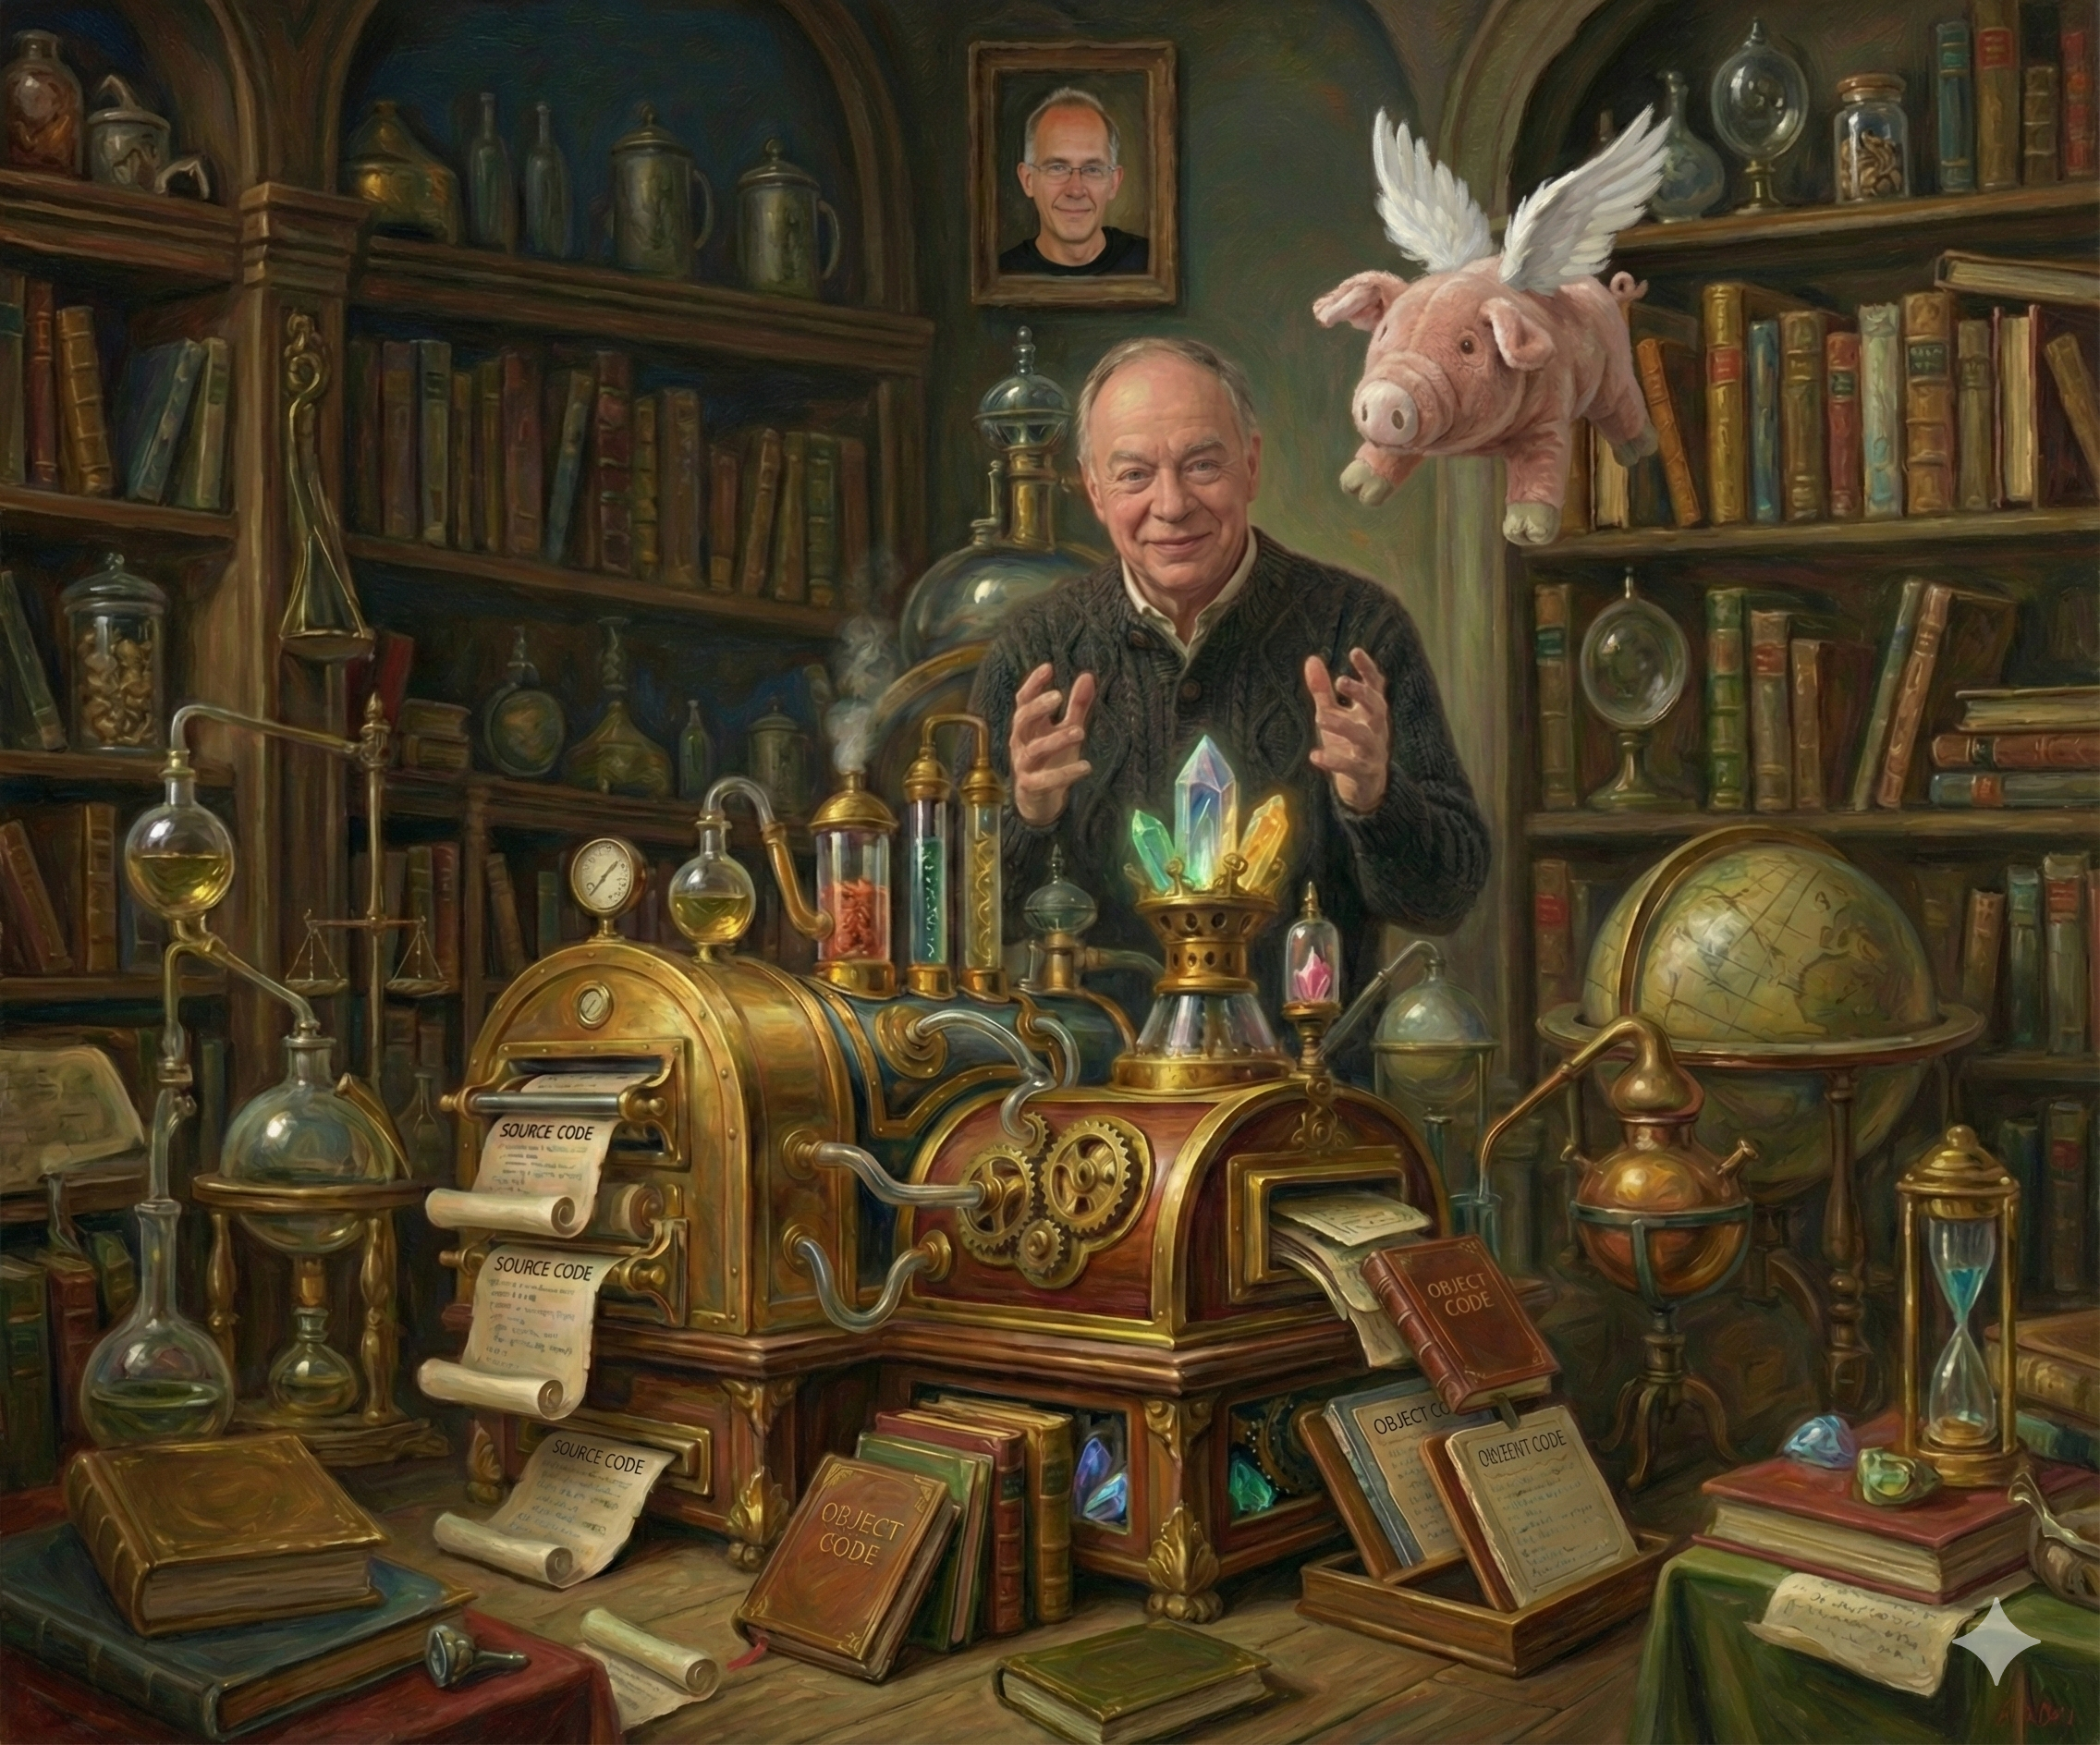
\includegraphics[width=17.0cm]{Abbildungen/compiler.jpg}
\caption{A medieval compiler.}
\label{fig:compiler.png}
\end{figure}

\noindent
In this chapter, we construct a compiler that translates a fragment of the \mytt{C} language into \textsl{Java}
assembler. The fragment of the \mytt{C} language translated by the compiler is referred to as
\blue{\textsl{Integer}-\mytt{C}}, \index{\textsl{Integer}-\mytt{C}} because only the data type \mytt{int} is
available. Although it would be feasible to support additional data types, the extra effort would no longer be
proportionate to the educational benefit of the example. 

A compiler essentially consists of the following components:
\begin{enumerate}
\item The scanner reads the file to be translated and breaks it down into a sequence of tokens. We will develop
      our scanner using the \simtextsc{Ply} tool. 
\item The parser reads the sequence of tokens and produces an abstract syntax tree as a result. We will 
      use \simtextsc{Ply} for the creation of the parser. 
\item The type-checker checks the abstract syntax tree for type errors. Since the language
      \textsl{Integer}-\mytt{C} contains only a single data type, this phase is not needed for our compiler. 
\item The code generator then translates the parse tree into a sequence of assembler commands that conform to
      the syntax of \textsl{Jasmin}. 
\item This can be followed by an \emph{optimization phase}.   Due to time constraints we cannot cover this
      topic. 
\item The resulting assembler program can be translated into Java bytecode using \textsl{Jasmin}.
\item The Java bytecode is then executed by the \simtextsc{Jvm}, i.e.~the \textsl{Java} virtual machine.
\end{enumerate}
In compilers whose target code is a \simtextsc{Risc} assembler program, a code similar to \simtextsc{Jvm} code is
usually generated first. Such a code is referred to as \emph{intermediate code}. It then remains the task of a
so-called \emph{backend} to generate an assembler program for a given processor architecture. The most
challenging task here is to find a register allocation for the variables, such that as many variables as
possible can be held in registers.  


\section{The Programming Language \textsl{Integer}-\mytt{C}}
\begin{figure}[!ht]
  \begin{center}
  \begin{minipage}[t]{12.5cm}
  \begin{eqnarray*}    
\textsl{program}      & \rightarrow & \;\textsl{function}\mytt{+} \\[0.2cm]
\textsl{function}     & \rightarrow & \quoted{int} \simtextsc{Id} \quoted{(} \textsl{paramList} \quoted{)} \quoted{\{} \textsl{decl}\,\mytt{+}\; \textsl{stmnt}\mytt{+} \;\squoted{\}} \\[0.2cm]
\textsl{paramList}    & \rightarrow & \;(\squoted{int}\, \simtextsc{Id}\; (\squoted{,}\, \quoted{int} \simtextsc{Id})\mytt{*})?  \\[0.2cm]
\textsl{decl}  & \rightarrow & \quoted{int} \simtextsc{Id} \quoted{;}  \\[0.2cm]
\textsl{stmnt}    & \rightarrow & \quoted{\{} \textsl{stmnt}\mytt{*} \quoted{\}}  \\[0.0cm]
                      & \mid        & \;\simtextsc{Id} \quoted{=} \textsl{expr} \;\squoted{;} \\[0.0cm]
                      & \mid        &  \quoted{if} \quoted{(} \textsl{boolExpr} \quoted{)} \textsl{stmnt} \\[0.0cm]
                     & \mid         &  \quoted{if} \quoted{(} \textsl{boolExpr} \quoted{)} \textsl{stmnt} \quoted{else} \textsl{stmnt} \\[0.0cm]
                     & \mid        &  \quoted{while} \quoted{(} \textsl{boolExpr} \quoted{)} \textsl{stmnt} \\[0.0cm]
                     & \mid        &  \quoted{return} \textsl{expr}\; \squoted{;} \\[0.0cm]
                     & \mid        &  \;\textsl{expr} \;\squoted{;}               \\[0.2cm]
   \textsl{boolExpr} & \rightarrow & \textsl{boolExpr} \;(\squoted{\&\&} \mid \squoted{||})\; \textsl{boolExpr} \\
         & \mid      &  \quoted{!} \textsl{boolExpr}             \\[0.0cm]
                     & \mid        &  \quoted{(} \textsl{boolExpr} \quoted{)}   \\[0.2cm]
         & \mid      &    \textsl{expr} \;(\squoted{==} \mid \squoted{!=} \mid \squoted{<=} \mid \squoted{>=} \mid \squoted{<} \mid \squoted{>})\;  \textsl{expr} \\[0.2cm]
 \textsl{expr} & \rightarrow & \textsl{expr} \;(\squoted{+} \mid \squoted{-} \mid \squoted{*} \mid \squoted{/} \mid \squoted{\%})\; \textsl{expr} \\[0.0cm]
     & \mid        &  \quoted{(} \textsl{expr} \quoted{)}                 \\[0.0cm]
     & \mid        &  \simtextsc{Number}                             \\[0.0cm]
     & \mid        &  \simtextsc{Id}\; (\squoted{(} (\textsl{expr}\; (\squoted{,}\; \textsl{expr})\mytt{*})?\;\squoted{)})?  
  \end{eqnarray*}
  \vspace*{-0.5cm}

  \end{minipage}
  \end{center}
  \caption{An \simtextsc{Ebnf} grammar for \textsl{Integer}-\textsc{C}}
\label{fig:compiler.ebnf}
\end{figure}

\noindent
We now introduce the language \textsl{Integer}-\texttt{C}, which our compiler is intended to translate. In this
context, we also refer to it as the \emph{source language} of our compiler. Figure \ref{fig:compiler.ebnf} on
page \pageref{fig:compiler.ebnf} shows the grammar of the source language in Extended Backus-Naur Form
(\simtextsc{Ebnf}). The grammar for \textsl{Integer}-\texttt{C} uses the following terminals: 
\begin{enumerate}
\item \simtextsc{Id} is an abbreviation for \blue{Identifier} and represents a sequence of digits, letters, and underscores that begins with a letter. An \simtextsc{Id} designates either a variable or the name of a function.
\item \simtextsc{Number} stands for a sequence of digits interpreted as a decimal number.
\item In addition, there are a number of operators such as \texttt{"+"}, \texttt{"-"}, etc., as well as keywords like \texttt{"if"}, \texttt{"else"}, and \texttt{"while"}.
\end{enumerate}
According to the grammar provided above, a program is a list of functions. A function consists of the
declaration of its signature, followed by a list of declarations (\textsl{decl}) and commands (\textsl{stmt})
enclosed in curly braces.  The grammar shown
in Figure \ref{fig:compiler.ebnf} is ambiguous:
\pagebreak

\begin{enumerate}
\item The grammar has the \blue{Dangling-Else Problem}.  We will solve this problem via operator precedences. 
\item For the operators used in arithmetic and Boolean expressions, precedences must be set to resolve
      ambiguities in the interpretation of these expressions. 
\end{enumerate}

\begin{figure}[!ht]
\centering
\begin{Verbatim}[ frame         = lines, 
                  framesep      = 0.3cm, 
                  labelposition = bottomline,
                  numbers       = left,
                  numbersep     = -0.2cm,
                  xleftmargin   = 0.8cm,
                  xrightmargin  = 0.8cm,
                ]
    int sum(int n) {
        int s;
        s = 0;
        while (n != 0) {
            s = s + n;
            n = n - 1;    
        };
        return s;
    }  
    int main() {
        int n;
        n = 6 * 6;
        println(sum(n));
    }
\end{Verbatim}
\vspace*{-0.3cm}
\caption{A simple \simtextsc{Integer}-\mytt{C} program to compute the sum
  $\displaystyle \sum\limits_{i=1}^{6 \cdot 6} i$.}
\label{fig:sum.c}
\end{figure}

\noindent
Figure \ref{fig:sum.c} shows a simple \simtextsc{Integer}-\texttt{C} program. The function $\textsl{sum}(n)$
calculates the sum 
\\[0.2cm]
\hspace*{1.3cm}
$\displaystyle\sum\limits_{i=1}^n i$
\\[0.2cm]
 and the function $\textsl{main}()$ calls the function \texttt{sum}
with the argument $6 \cdot 6$. The function \texttt{println} used in the program outputs its argument followed
by a newline. We assume that this function is predefined. 

\section{Developing the  Scanner and the Parser}
We construct both the scanner and the parser using  \textsl{Ply}.
Figure \ref{fig:Compiler.ipynb:lex} shows the scanner.  The scanner
recognizes the operators, keywords, identifiers, and numbers.  As the scanner is mostly similar to those
scanners that we have already seen before, there are only a few points worth mentioning.

\begin{figure}[!ht]
\centering
\begin{minted}[ frame        = lines, 
                framesep     = 0.3cm, 
                bgcolor      = sepia,
                numbers      = left,
                numbersep    = -0.2cm,
                xleftmargin  = 0.0cm,
                xrightmargin = 0.0cm,
              ]{python3}
   import ply.lex as lex
   
   tokens = [ 'NUMBER', 'ID', 'EQ', 'NE', 'LE', 'GE', 'AND', 'OR',
              'INT', 'IF', 'ELSE', 'WHILE', 'RETURN'             ]

   t_NUMBER = r'0|[1-9][0-9]'
   t_EQ  = r'=='
   t_NE  = r'!='
   t_LE  = r'<='
   t_GE  = r'>='
   t_AND = r'&&'
   t_OR  = r'\|\|'
   
   def t_COMMENT(t):
       r'//[^\n]*'
       pass

   Keywords = { 'int': 'INT', 'if': 'IF', 'else': 'ELSE', 
                'while': 'WHILE', 'return': 'RETURN'      }
   
   def t_ID(t):
       r'[a-zA-Z][a-zA-Z0-9_]*'
       t.type = Keywords.get(t.value, 'ID')
       return t
   
   literals = ['+', '-', '*', '/', '%', '(', ')', '{', '}', 
               '=', '<', '>', '!', ',', ';'                 ]
   
   t_ignore  = ' \t\r'
   
   def t_newline(t):
       r'\n+'
       t.lexer.lineno += t.value.count('\n')

   def t_error(t):
       print(f"Illegal character '{t.value[0]}' in line {t.lineno}.")
       t.lexer.skip(1)
   
   __file__ = 'main'    
   lexer    = lex.lex()
\end{minted}
\vspace*{-0.3cm}
\caption{The scanner for \textsl{Integer}-\mytt{C}.}
\label{fig:Compiler.ipynb:lex}
\end{figure}

\begin{enumerate}
\item If a token does not have to be manipulated by the scanner, then it can be defined by a simple equation 
      of the form 
      \\[0.2cm]
      \hspace*{1.3cm}
      \mytt{t\_\textsl{name} = \textsl{regexp}}
      \\[0.2cm]
      where \textsl{name} is the name of the token and \textsl{regexp} is the regular expression defining the
      token.  We have used this shortcut to define most of the tokens recognized by our scanner.
\item While we do not need to declare tokens for those operators that consist of just one token, 
      we have to declare those tokens that consist of two or more characters.  For example, the operator
      \quoted{==} is represented by the token \mytt{'EQ'} and is defined in line 7.
\item Our programming language supports single line comments that start with the string \quoted{//} and extend
      to the end of the line.  These comments are implemented via the token \mytt{COMMENT} that is defined in
      line 14--16.  Note that the function \mytt{t\_COMMENT} does not return a value.  Therefore,
      these comments are simply discarded.  This is also the reason that we have to use a function to define
      this token.
\item The most interesting aspect is the implementation of keywords like \quoted{while} or \quoted{return}.
      Note that we have defined separate tokens for all of the keywords but we have not defined any
      of these tokens.  For example, we have not defined \mytt{t\_return}.
      The reason is that, syntactically, all of the keywords are identifiers and are recognized by the regular
      expression
      \\[0.2cm]
      \hspace*{1.3cm}
      \mytt{r'[a-zA-Z][a-zA-Z0-9\_]*'}
      \\[0.2cm]
      that is used for recognizing identifiers in line 22.  However, the function \mytt{t\_ID} that recognizes
      identifiers does not immediately return the token \mytt{'ID'} when it has scanned the name of an
      identifier.  Rather, it first checks whether this name is a predefined keyword.  The predefined keywords
      are the key of the dictionary \mytt{Keywords} that is defined in line 18 and 19.  The values of the
      keywords in this dictionary are the token types.  Therefore, the function \mytt{t\_ID} sets the
      \blue{token type} of the token that is returned to the value stored in the dictionary \mytt{Keywords}.
      In case a name is not defined in this dictionary, the token type is set to \mytt{'ID'}.
\item The scanner implements the function \mytt{t\_newline} in line 31.  This function is needed
      to update the attribute \mytt{lineno} of the scanner.  This attribute stores the line number and is
      needed for error messages.
\end{enumerate}

\begin{figure}[!ht]
\centering
\begin{minted}[ frame        = lines, 
                framesep     = 0.3cm, 
                bgcolor      = sepia,
                numbers      = left,
                numbersep    = -0.2cm,
                xleftmargin  = -0.5cm,
                xrightmargin = -0.3cm,
              ]{python3}
  import ply.yacc as yacc
  
  start = 'program'
  
  precedence = (
      ('nonassoc', 'IF'),
      ('nonassoc', 'ELSE'),
      ('left', 'OR'),
      ('left', 'AND'),
      ('right', '!'),
      ('nonassoc', 'EQ', 'NE', 'LE', 'GE', '<', '>'),
      ('left', '+', '-'),
      ('left', '*', '/', '%')
  )
  
  def p_program_one(p):
      "program : function"
      p[0] = ('.', p[1])
      
  def p_program_more(p):
      "program : function program"
      p[0] = ('.', p[1]) + p[2][1:]
  
  def p_function(p):
      "function : INT ID '(' param_list ')' '{' decl_list stmnt_list '}'"
      p[0] = ('fct', p[2], p[4], p[7], p[8])
\end{minted}
\vspace*{-0.3cm}
\caption{Grammar for Integer-\texttt{C}, part 1.}
\label{fig:Compiler.ipynb-1}
\end{figure}

Now we are ready to present the specification of our parser.  For reasons of space,
we have split the grammar into six parts.  We start with Figure \ref{fig:Compiler.ipynb-1} on page
\pageref{fig:Compiler.ipynb-1}.  
\begin{enumerate}
\item Line 3 declares the start symbol \mytt{program}.
\item Line 5--14 declare the operator precedences.
  \begin{enumerate}[(a)]
  \item The keywords ``\mytt{if}'' and ``\mytt{else}''  have the lowest precedence and the precedence of
        ``\mytt{if}'' is lower than the precedence of ``\mytt{else}''.  This is necessary to solve the
        \blue{dangling else} conflict.
  \item The operator ``\mytt{||}'' that represents \blue{logical or} has the lowest precedence of all proper
        operators and associates to the left.  
  \item The operator ``\mytt{\&\&}'' that represents \blue{logical and} binds stronger than ``\mytt{||}''
        but not as strong as  the negation operator ``\mytt{!}''.
  \item The negation operator ``\mytt{!}'' is right associative because we want to interpret an expression of
        the form $\mytt{!!}a$ as  $\mytt{!}(\mytt{!}a)$.
  \item The comparison operators ``\mytt{==}'', ``\mytt{!=}'', ``\mytt{<=}'', ``\mytt{>=}'',
        ``\mytt{<}'', and ``\mytt{>}'' are non-associative, since our programming languages disallows 
        the chaining of comparison operators, i.e.~an expression of the form $x < y < z$ is syntactically
        invalid.
  \item The arithmetical operators ``\mytt{+}'' and ``\mytt{-}'' have a lower precedence than the
        arithmetical operators ``\mytt{*}'', ``\mytt{/}'',  and ``\mytt{\%}''. 
  \end{enumerate}
\item A \mytt{program} is a non-empty list of \mytt{function} definitions.  Therefore, it is either a single
      function definition (line 16--18) or it is a function definition followed by more function definitions
      (line 20--22).

      The purpose of the parser is to turn the given program into an abstract syntax tree.  This abstract
      syntax tree is represented as a \blue{nested tuple}.  A program consisting of the functions 
      $f_1$, $\cdots$, $f_n$ is represented as the nested tuple.
      \\[0.2cm]
      \hspace*{1.3cm}
      $(\squoted{program}, f_1, \cdots, f_n)$.
      \\[0.2cm] 
      If in line 19 a \mytt{program} consisting of a \mytt{function} and another \mytt{program} is
      parsed, the expression \mytt{p[2]} in line 20 refers to the abstract syntax tree representing the
      \mytt{program} that follows the \mytt{function}.  The expression \mytt{p[2][1:]} discards the
      keyword \squoted{program} that is at the start of this nested tuple.  Hence,  \mytt{p[2][1:]}
      is just a tuple of the functions following the first \mytt{function}.  Therefore, the assignment to \mytt{p[0]}
      creates a nested tuple that starts with the keyword \squoted{program} followed by all the functions
      defined in this program.
\item A \mytt{function} definition starts with the keyword \squoted{int} that is followed by the name of the
      function, an opening parenthesis, a list of the parameters of the function, a closing parenthesis,
      an opening brace, a list of declarations, a list of statements, and finally a closing brace.

      The initial version of the programming language \texttt{C}, as detailed in the book
      ``\emph{The C Programming Language}'' \cite{kernighan:1978}, required that all variable declarations
      precede any statements, prohibiting the mixing of declarations and statements. While this limitation was
      lifted in subsequent versions of the language, our implementation still enforces this restriction.       
\end{enumerate}

\begin{figure}[!ht]
\centering
\begin{minted}[ frame        = lines, 
                framesep     = 0.3cm, 
                bgcolor      = sepia,
                numbers      = left,
                firstnumber  = last,
                numbersep    = -0.2cm,
                xleftmargin  = 0.8cm,
                xrightmargin = 0.8cm,
              ]{python3}
    def p_param_list_empty(p):
        "param_list :"
        p[0] = ('.', )
        
    def p_param_list_one(p):
        "param_list : INT ID"
        p[0] = ('.', p[2])
        
    def p_param_list_more(p):
        "param_list : INT ID ',' ne_param_list"
        p[0] = ('.', p[2]) + p[4][1:]
    
    def p_ne_param_list_one(p):
        "ne_param_list : INT ID"
        p[0] = ('.', p[2])
        
    def p_ne_param_list_more(p):
        "ne_param_list : INT ID ',' ne_param_list"
        p[0] = ('.', p[2]) + p[4][1:]
    
    def p_decl_list_empty(p):
        "decl_list :"
        p[0] = ('.',)
    
    def p_decl_list_more(p):
        "decl_list : INT ID ';' decl_list"
        p[0] = ('.', p[2]) + p[4][1:]
    
    def p_stmnt_list_empty(p):
        "stmnt_list :"
        p[0] = ('.',)
    
    def p_stmnt_list_more(p):
        "stmnt_list : stmnt stmnt_list"
        p[0] = ('.', p[1]) + p[2][1:]
\end{minted}
\vspace*{-0.3cm}
\caption{ Grammar for Integer-\texttt{C}, part 2.}
\label{fig:Compiler.ipynb-2}
\end{figure}

Figure \ref{fig:Compiler.ipynb-2} shows the definition of parameter lists, declaration lists, and statement lists.
\begin{enumerate}
\item The definition of a list of parameters is quite involved, because parameter lists may be empty and,
      furthermore, different parameters have to be separated by \squoted{,}.  Therefore, we have to introduce 
      the additional syntactical variable \mytt{ne\_param\_list}, which represents a non-empty parameter
      list.  The grammar rules for \mytt{param\_list} are as follows:
      \pagebreak
      
      \begin{verbatim}
        param_list 
             : /* epsilon */
             | 'int' ID
             | 'int' ID ',' ne_param_list
             ;
        ne_param_list 
             : 'int' ID
             | 'int' ID ',' ne_param_list
             ;
      \end{verbatim}
      We use the \quoted{.} as a key to represent lists of any kind as nested tuples.
\item The grammar rules for a list of declarations are as follows:
      \begin{verbatim}
      decl_list
          : /* epsilon */
          | 'int' ID ';' decl_list
          ;
      \end{verbatim}
      Observe that with this definition a list of declarations may be empty.
      The grammar rules for a list of declarations are simpler than the grammar rules for a parameter list
      because every variable declaration is ended with a semicolon, while parameters are separated by commas
      and the last parameter must not be followed by a comma.
\item The grammar rules for a list of statements are as follows:
      \begin{verbatim}
      stmnt_list
          : /* epsilon */
          | stmnt stmnt_list
          ;
      \end{verbatim}
\end{enumerate}
\begin{figure}[!ht]
\centering
\begin{minted}[ frame        = lines, 
                framesep     = 0.3cm, 
                bgcolor      = sepia,
                numbers      = left,
                firstnumber   = last,
                numbersep    = -0.2cm,
                xleftmargin  = 0.8cm,
                xrightmargin = 0.8cm,
              ]{python3}
    def p_stmnt_block(p):
        "stmnt : '{' stmnt_list '}'"
        p[0] = p[2]
        
    def p_stmnt_assign(p):
        "stmnt : ID '=' expr ';'"
        p[0] = ('=', p[1], p[3])
        
    def p_stmnt_if(p):
        "stmnt : IF '(' bool_expr ')' stmnt"
        p[0] = ('if', p[3], p[5])   
        
    def p_stmnt_if_else(p):
        "stmnt : IF '(' bool_expr ')' stmnt ELSE stmnt"
        p[0] = ('if-else', p[3], p[5], p[7])
        
    def p_stmnt_while(p):
        "stmnt : WHILE '(' bool_expr ')' stmnt"
        p[0] = ('while', p[3], p[5])
        
    def p_stmnt_return(p):
        "stmnt : RETURN expr ';'"
        p[0] = ('return', p[2])
        
    def p_stmnt_expr(p):
        "stmnt : expr ';'"
        p[0] = p[1]
\end{minted}
\vspace*{-0.3cm}
\caption{Grammar for Integer-\texttt{C}, part 3.}
\label{fig:Compiler.ipynb-3}
\end{figure}

\noindent
Figure \ref{fig:Compiler.ipynb-3} on page \pageref{fig:Compiler.ipynb-3} shows how the variable \mytt{stmnt} is
defined.  The grammar rules for statements are as follows:
\begin{verbatim}
        stmnt : '{' stmnt_list '}'
              | ID '=' expr ';'
              | 'if' '(' bool_expr ')' stmnt
              | 'if' '(' bool_expr ')' stmnt 'else' stmnt
              | 'while' '(' bool_expr ')' stmnt
              | 'return' expr ';'
              | expr ';'
              ;
\end{verbatim}

\begin{figure}[!ht]
\centering
\begin{minted}[ frame        = lines, 
                framesep     = 0.3cm, 
                bgcolor      = sepia,
                numbers      = left,
                firstnumber  = last,
                numbersep    = -0.2cm,
                xleftmargin  = 0.8cm,
                xrightmargin = 0.8cm,
              ]{python3}
    def p_bool_expr_or(p):
        "bool_expr : bool_expr OR bool_expr"
        p[0] = ('||', p[1], p[3])
        
    def p_bool_expr_and(p):
        "bool_expr : bool_expr AND bool_expr"
        p[0] = ('&&', p[1], p[3])
    
    def p_bool_expr_neg(p):
        "bool_expr : '!' bool_expr"
        p[0] = ('!', p[2])

    def p_bool_expr_paren(p):
        "bool_expr : '(' bool_expr ')'"
        p[0] = p[2]

    def p_bool_expr_eq(p):
        "bool_expr : expr EQ expr"
        p[0] = ('==', p[1], p[3])
    
    def p_bool_expr_ne(p):
        "bool_expr : expr NE expr"
        p[0] = ('!=', p[1], p[3])
    
    def p_bool_expr_le(p):
        "bool_expr : expr LE expr"
        p[0] = ('<=', p[1], p[3])
        
    def p_bool_expr_ge(p):
        "bool_expr : expr GE expr"
        p[0] = ('>=', p[1], p[3])
        
    def p_bool_expr_lt(p):
        "bool_expr : expr '<' expr"
        p[0] = ('<', p[1], p[3])
    
    def p_bool_expr_gt(p):
        "bool_expr : expr '>' expr"
        p[0] = ('>', p[1], p[3])
\end{minted}
\vspace*{-0.3cm}
\caption{Grammar for Integer-\texttt{C}, part 4.}
\label{fig:Compiler.ipynb-4}
\end{figure}

\noindent
Figure \ref{fig:Compiler.ipynb-4} on page \pageref{fig:Compiler.ipynb-4} shows how Boolean expressions are
defined.  The grammar rules are as follows:
\pagebreak

\begin{verbatim}
        bool_expr : bool_expr '||' bool_expr
                  | bool_expr '&&' bool_expr
                  | '!' bool_expr
                  | '(' bool_expr ')'
                  | expr '==' expr
                  | expr '!=' expr
                  | expr '<=' expr
                  | expr '>=' expr
                  | expr '<'  expr
                  | expr '>'  expr
                  ;
\end{verbatim}

\begin{figure}[!ht]
\centering
\begin{minted}[ frame        = lines, 
                framesep     = 0.3cm, 
                bgcolor      = sepia,
                numbers      = left,
                firstnumber  = last,
                numbersep    = -0.2cm,
                xleftmargin  = 0.8cm,
                xrightmargin = 0.8cm,
              ]{python3}
    def p_expr_plus(p):
        "expr : expr '+' expr"
        p[0] = ('+', p[1], p[3])
        
    def p_expr_minus(p):
        "expr : expr '-' expr"
        p[0] = ('-', p[1], p[3])
        
    def p_expr_times(p):
        "expr : expr '*' expr"
        p[0] = ('*', p[1], p[3])
        
    def p_expr_divide(p):
        "expr : expr '/' expr"
        p[0] = ('/', p[1], p[3])
        
    def p_expr_modulo(p):
        "expr : expr '%' expr"
        p[0] = ('%', p[1], p[3])

    def p_expr_group(p):
        "expr : '(' expr ')'"
        p[0] = p[2]
    
    def p_expr_number(p):
        "expr : NUMBER"
        p[0] = ('Number', p[1])
    
    def p_expr_id(p):
        "expr : ID"
        p[0] = p[1]
        
    def p_expr_fct_call(p):
        "expr : ID '(' expr_list ')'"
        p[0] = ('call', p[1]) + p[3][1:]
\end{minted}
\vspace*{-0.3cm}
\caption{Grammar for Integer-\texttt{C}, part 5.}
\label{fig:Compiler.ipynb-5}
\end{figure}
\noindent
Figure \ref{fig:Compiler.ipynb-5} on page \pageref{fig:Compiler.ipynb-5} shows how arithmetic expressions
are defined.  The grammar rules are as follows:
\pagebreak
\vspace*{\fill}

\pagebreak
\vspace*{\fill}

\pagebreak

\begin{verbatim}
        expr : expr '+' expr
             | expr '-' expr
             | expr '*' expr
             | expr '/' expr
             | expr '%' expr
             | '(' expr ')'
             | NUMBER
             | ID
             | ID '(' expr_list ')'
\end{verbatim}

\noindent
Finally, Figure \ref{fig:Compiler.ipynb-6} on page \pageref{fig:Compiler.ipynb-6} shows how \mytt{expr\_list}
is defined.  
\begin{verbatim}
        expr_list : /* epsilon */
                  | expr
                  | expr ',' ne_expr_list
                  ;

        ne_expr_list : expr
                     | expr ',' ne_expr_list
                     ;
\end{verbatim}
Furthermore, this function shows the definition of the function \mytt{p\_error}, which is called if
\simtextsc{Ply} detects a syntax error.  \simtextsc{Ply} will detect a syntax error in the case that the state of the
generated shift/reduce parser has no action for the next input token.  The argument \mytt{p} to the function
\mytt{p\_error} is the first token for which the action of the shift/reduce parser is undefined.
In this case \mytt{p.value} is the part of the input string corresponding to this token.

\begin{figure}[!ht]
\centering
\begin{minted}[ frame        = lines, 
                framesep     = 0.3cm, 
                bgcolor      = sepia,
                numbers      = left,
                firstnumber  = last,
                numbersep    = -0.2cm,
                xleftmargin  = -0.5cm,
                xrightmargin = 0.0cm,
              ]{python3}
  def p_expr_list_empty(p):
      "expr_list :"
      p[0] = ('.',)
      
  def p_expr_list_one(p):
      "expr_list : expr"
      p[0] = ('.', p[1])     
  
  def p_expr_list_more(p):
      "expr_list : expr ',' ne_expr_list"
      p[0] = ('.', p[1]) + p[3][1:]     
  
  def p_ne_expr_list_one(p):
      "ne_expr_list : expr"
      p[0] = ('.', p[1]) 
      
  def p_ne_expr_list_more(p):
      "ne_expr_list : expr ',' ne_expr_list"
      p[0] = ('.', p[1]) + p[3][1:] 
  
  def p_error(p):
      if p:
          print(f'Syntax error at "{p.value}" in line {p.lineno}.')
      else:
          print('Syntax error at end of input.')
  
  parser = yacc.yacc(write_tables=False, debug=True)
\end{minted}
\vspace*{-0.3cm}
\caption{Grammar for Integer-\texttt{C}, part 6.}
\label{fig:Compiler.ipynb-6}
\end{figure}

\exerciseEng
Extend the parser that is available at
\\[0.2cm]
\hspace*{1.3cm}
\href{
 https://github.com/karlstroetmann/Formal-Languages/blob/master/Ply/Compiler.ipynb}{https://github.com/karlstroetmann/Formal-Languages/blob/master/Ply/Compiler.ipynb} 
\\[0.2cm]
so that it supports the ternary \texttt{C}-operator for conditional expressions.  For example, in \texttt{C},
the following assignment using the ternary operator can be used to assign to the variable \mytt{max}
the maximum of the values of the variables \mytt{x} and \mytt{y}:
\\[0.2cm]
\hspace*{1.3cm}
\mytt{max = x > y ? x : y;}
\\[0.2cm]
Extend the parser so it can process the assignment shown above. \eox 

%%% Local Variables: 
%%% mode: latex
%%% TeX-master: "formal-languages"
%%% End: 
